% Figure 1: shared verification root and silent inheritance (EuroSys problem architecture)
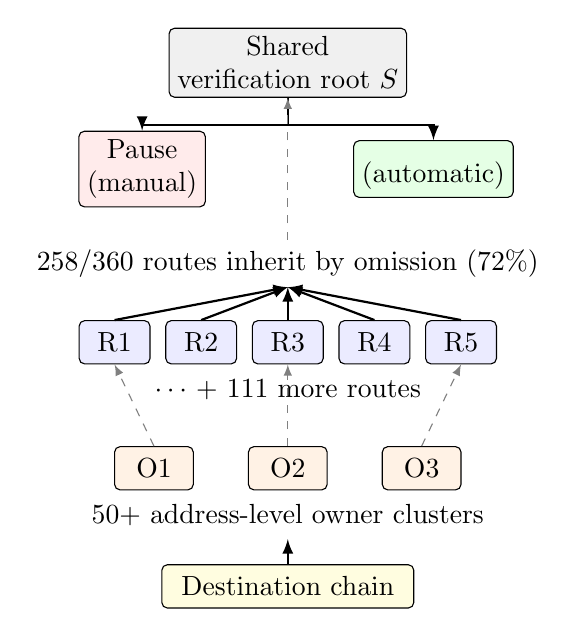
\begin{tikzpicture}[
  font=\normalsize,
  box/.style={draw, rounded corners=2pt, align=center, inner sep=3pt, minimum height=0.55cm},
  small/.style={box, minimum width=1.45cm},
  root/.style={box, fill=gray!12, minimum width=2.5cm},
  route/.style={box, fill=blue!8, minimum width=0.9cm},
  op/.style={box, fill=orange!10, minimum width=1.0cm},
  arr/.style={->, >=latex, thick},
  dasharr/.style={->, >=latex, dashed, gray}
]
  \node[root] (root) at (0,0) {Shared\\verification root $S$};
  \node[small, fill=red!8] (pause) at (-1.85,-1.35) {Pause\\(manual)};
  \node[small, fill=green!10] (budget) at (1.85,-1.35) {\sys\\(automatic)};
  \draw[arr] (root.south) -- ++(0,-0.35) -| (pause.north);
  \draw[arr] (root.south) -- ++(0,-0.35) -| (budget.north);

  \node[align=center] (inherit) at (0,-2.55)
    {258/360 routes inherit by omission (72\%)};
  \draw[dasharr] (inherit.north) -- (root.south);

  \foreach \x/\lab in {-2.2/R1, -1.1/R2, 0/R3, 1.1/R4, 2.2/R5} {
    \node[route] (r\lab) at (\x,-3.55) {\lab};
    \draw[arr] (r\lab.north) -- (inherit.south);
  }
  \node at (0,-4.15) {$\cdots$ + 111 more routes};

  \foreach \x/\lab in {-1.7/O1, 0/O2, 1.7/O3} {
    \node[op] (o\lab) at (\x,-5.15) {\lab};
  }
  \node[align=center] at (0,-5.75) {50+ address-level owner clusters};
  \draw[dasharr] (oO1.north) -- (rR1.south);
  \draw[dasharr] (oO2.north) -- (rR3.south);
  \draw[dasharr] (oO3.north) -- (rR5.south);

  \node[box, fill=yellow!12, minimum width=3.2cm] (dest) at (0,-6.65) {Destination chain};
  \draw[arr] (dest.north) -- (0,-6.05);

\end{tikzpicture}
